\section{BE21B040}
\begin{center}
    \textbf{\Large{Growth Curve and Generation Time of Bacteria}} \\
    \normalsize{Sumedh Kangne, BE21B040} \\
    \normalsize{22 June, 2022}
\end{center}

\textbf{\Large{Introduction}} \\

A Bacterial culture is know to have an exponential growth curve under favorable conditions. It doubles every generation following a geometric progression like $2^0,2^1,2^2,2^3,.......,2^n$ (where n=number of generations). Although, this exponential growth phase is only a part of the entire process. \\

\textbf{\Large{Characteristic Growth Phases:}} \\

There are 4 growth phases:

\begin{enumerate}
    \item \textbf{Lag Phase :} This is a phase where there is no significant growth in the number of bacteria in the sample. This phase is kind of the preparatory phase for the bacteria. They undergo all sorts of metabolic activities such as synthesis of enzymes, proteins, RNA, recovering from the wear and tear the cells have faced etc.
    
    \item \textbf{Exponential (log) Phase :} This is the phase where the bacteria undergo a binary fission and grow exponentially. We calculate the rate in terms of the Generation time \textbf{G} which is equal to time taken \textbf{t} upon the number of generations \textbf{n}. Therefore
    \begin{equation}
        \textbf{G}=\textbf{t/n}
        \label{eqn:generationTime}
    \end{equation}
    
    \item \textbf{Stationary Phase :} In this phase the Growth in the number of bacteria comes to a still. This maybe because of three reasons:
    \begin{itemize}
        \item Exhaustion of nutrients
        \item Running out of space
        \item Accumulation of inhibitory metabolites
    \end{itemize}
    
    \item \textbf{Death Phase :} During this phase the number of viable cells decrease exponentially, similar to log phase.

    \begin{center}
		\framebox{
			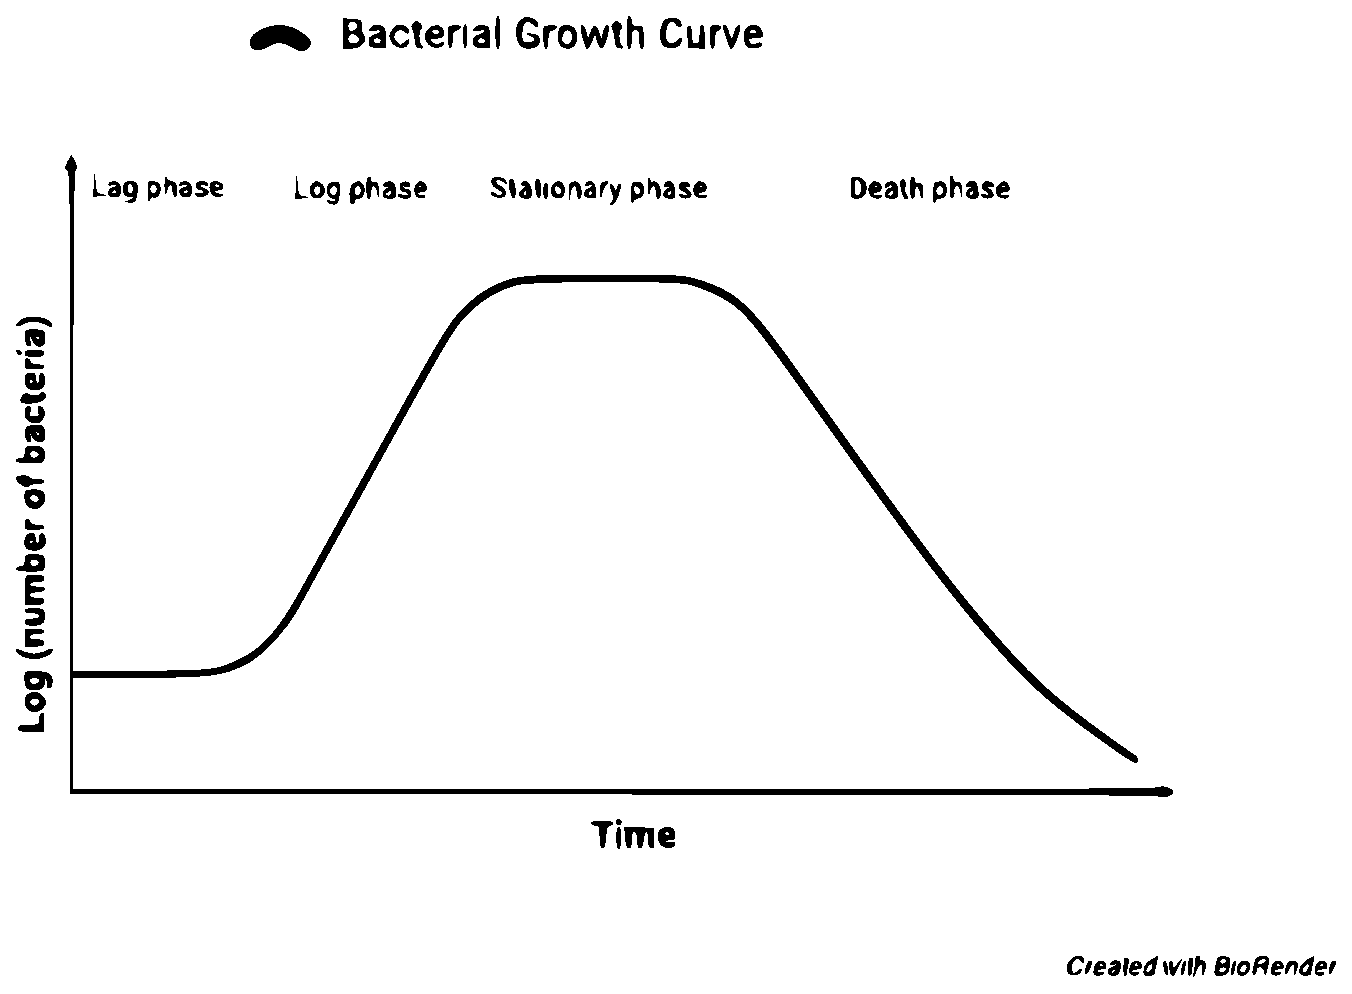
\includegraphics[scale=0.3]{BE21B040/BacterialGrowthGraph.eps}
		}
	\end{center}
	
\end{enumerate} 
\textbf{\Large{Calculation of Generation time}} \\

Generation time is the time taken by the bacteria to double in number as in the previous generation or in simpler terms undergo one binary fission. Common examples such as E. coli have a generation time of 17 minutes in a medium of glucose-salts.

\begin{table}[h]
	\begin{center}
\begin{tabular}{|c|l|}
\hline
	Variables & Description \\
\hline
	$N_0$ & Initial number of bacteria \\
	$N$ & Final number of bacteria \\
	$G$ & Generation time \\
	$n$ & Number of generations \\
	$t$ & Total time period \\
\hline
\end{tabular}
	\caption{Table of variables used in the equation}
	\label{tab:varTimeTable}
	\end{center}
\end{table}

	\[{N} = {N_0}\times{2^n}\]
	Solving for n:
	\[\log{N} = \log{N_0}+{n}\log{2}\]
	\[{n} = \frac{\log{N}-\log{N_0}}{log{2}}\]
    \[{n} = \frac{\log{N}-\log{N_0}}{0.301}\]
    \[{n} = {3.3}\log({\frac{N}{N_0}})\]
    Using eq \ref{eqn:generationTime},
    \[{G} = \frac{t}{n}\]
    \begin{equation}
        {G} = \frac{t}{{3.3}\log({\frac{N}{N_0}})}
    \end{equation}
    
    
\nocite{*}
\bibliography{biblio}
\bibliographystyle{alpha}
